\documentclass[letterpaper,twocolumn,10pt]{article}
\usepackage{usenix,epsfig,endnotes}

%%%%%%%%%%%%%%%%%%%%%%%%%%%%% DELETE AFTER %%%%%%%%%%%%%%%%%%%%%%%%%%%%%%%%%%%%
\usepackage{lipsum}
\usepackage{xargs}                      % Use more than one optional parameter in a new commands
\usepackage[pdftex,dvipsnames]{xcolor}
\usepackage[colorinlistoftodos,prependcaption,textsize=tiny]{todonotes}
\newcommandx{\unsure}[2][1=]{\todo[linecolor=red,backgroundcolor=red!25,bordercolor=red,#1]{#2}}
\newcommandx{\change}[2][1=]{\todo[linecolor=blue,backgroundcolor=blue!25,bordercolor=blue,#1]{#2}}
\newcommandx{\info}[2][1=]{\todo[linecolor=OliveGreen,backgroundcolor=OliveGreen!25,bordercolor=OliveGreen,#1]{#2}}
\newcommandx{\improvement}[2][1=]{\todo[linecolor=Plum,backgroundcolor=Plum!25,bordercolor=Plum,#1]{#2}}
\newcommandx{\thiswillnotshow}[2][1=]{\todo[disable,#1]{#2}}
\setlength{\marginparwidth}{2cm}
%%%%%%%%%%%%%%%%%%%%%%%%%%%%%%%%%%%%%%%%%%%%%%%%%%%%%%%%%%%%%%%%%%%%%%%%%%%%%%%%%
\usepackage[none]{hyphenat}
\let\origref\ref
\def\ref#1{\textbf{\origref{#1}}}







%%%%%%%%%%%%%%%%%%%%%%%%%%%%%%%%%%%%%%%%%%%%%%%%BEGIN%%%%%%%%%%%%%%%%%%%%%%%%%%%%%%%%%%%%%%%
\begin{document}

%don't want date printed
\date{}
\title{\Large \bf Towards Fog-aware Kubernetes}
\author{
{\rm Ali J. Fahs}\\
Univ Rennes, CNRS, IRISA\\
ali.fahs@irisa.fr
\and
{\rm Guillaume Pierre}\\
Univ Rennes, Inria, CNRS, IRISA\\
guillaume.pierre@irisa.fr
}
\maketitle
\thispagestyle{empty}


\subsection*{Abstract}
Your Abstract Text Goes Here.  Just a few facts.Whet our appetites.
Keep it short. According to the APA style manual, an abstract should be between 150 to 250 words Keep it short. According to the APA style manual, an abstract should be between 150 to 250 words Keep it short. According to the APA style manual, an abstract should be between 150 to 250 words  According to the APA style manual, an abstract should be between 150 to 250 words Keep it short. According to the APA style manual, an abstract should be between 150 to 250 words 
%%%%%%%%%%%%%%%%%%%%%%%%%%%%%%%%%%%%%%%%%%%%%%%%%%%%%%%%%%% INTRODUCTION %%%%%%%%%%%%%%%%%%%%%%%%%%%%%%%%%%%%%%%%%%%%%%%%%%%
\section{Introduction}
%The introduction of Fog computing. DONE
\hskip .7em In a world where centralized data centres have been proven to be cost-effective, the big players of cloud services are relaying on more than a few data centres to serve millions of users all-over the globe. 

Such a model have seen the light due to the lack of interest in locating the services in a specific geolocation. 

 The user's applications can run in any server regardless of the location, and the communication between the user and the server is done through internet connections.\unsure{maybe i will remove this} The location of the data centres are chosen according to some factors like power cost, disregarding the impact on the end-to-end latency of the service. Furthermore, the cloud service user is not informed about the location of the server, where this location awareness is sometimes vital for specific types of application {\em (e.g., IoT applications)}.\change{language check and rephrase}

%The separation was not limited to the management alone, but also to the geographical location. 

Nowadays, some applications require lower latencies and location awareness. These requirments will be provided by an extended extended paradigm of cloud computing called Fog computing\cite{bonomi2011connected,Bonomi:2012:FCR:2342509.2342513}.

%The resource Fog provide.
The Fog computing is defined as an intermediary platform between the end devices and the cloud computing data centres. This platform provides compute, storage and networking resources,similar to clouds. Yet, the difference lies in the proximity to the user, low latency, distribution, and location awareness. 

%Fog targeted application and user proximity.
Unlike clouds which relies in a handful of resources rich data-centres, fog is based on the idea of spreading plenty points of presence in the proximity of the user. Since the end devices are close to the source, the latency can be significantly reduced, which will improve the users' experience. All of this can be done while considering the location of the access point as an important measure of the workload scheduling.

%Platforms for fog.
Since the concept of fog is relatively new, no platform was designed to assist fog architecture. However, a fog computing cluster can be deployed on top of cloud platforms like Docker swarm, Mesos, and Kubernetes.

%Kubernetes and Clouds.
For our cluster we have chosen Kubernetes for the reasons that will be mentioned in the paper.\change{link para}

%Why Kubernetes is not compatible with Fog computing (briefly).
Although Kubernetes provide automation and some source of load-balancing, still it doesn't have all the features to full-fill the definition of fog computing.    

%paper objective 
In this paper, we contribute a roadmap toward enabling a fog-aware Kubernetes.\change{definitely rephrase!}


%Explain organization of the report, what is included, and what is not.
This paper is organised as follows. In section \ref{plat} we briefly acknowledge the possible fog computing platforms. In section \ref{kube} we introduce Kubernetes as a platform, discuss the advantage and disadvantages in the context of fog. In section 
\ref{road} we demonstrate our vision through a roadmap of the steps that should be taken to achieve fog-aware Kubernetes. In the last section we conclude.\change{add something to the conclude}\unsure{long style style is ok ?} 


%%%%%%%%%%%%%%%%%%%%%%%%%%%%%%%%%%%%%%%%%%%%%%%%%%%%%%%%%%% Fog Computing %%%%%%%%%%%%%%%%%%%%%%%%%%%%%%%%%%%%%%%%%%%%%%%%%%%
\section{Fog Computing Platforms}\label{plat}
\hskip .5em For the fog architecture to function a set of infrastructure management tools are mandatory. In our search for the ideal platform we have focused on the ones that support containers, for the lightweight and portability containers offer over Virtual Machines(VM). 

The container orchestration Engines can be summed up by the three most used ones: Docker swarm, Mesos, and Kubernetes (K8's). All of these platforms provide container scheduling, cluster management, and support for large-scale clusters. 

We have chosen Kubernetes for our cluster and our development for the added features it offers like auto-scaling, load balancing, the concept of a Kubernetes service, the concept of pods, and ingress. Due to Kubernetes large community, it requires less third-party software, since most of the add-on features are already integrated. \unsure{do I have to mention openstack}\change{Maybe i need to write more}\change{rephrasing is a must}

\info{writing a small para for Picasso }
  
%%%%%%%%%%%%%%%%%%%%%%%%%%%%%%%%%%%%%%%%%%%%%%%%%%%%%%%%%%% Kubernetes %%%%%%%%%%%%%%%%%%%%%%%%%%%%%%%%%%%%%%%%%%%%%%%%%%%
\section{Kubernetes and Fog Computing}\label{kube}

\subsection{Kubernetes Architecture}
%\begin{figure}[th]

%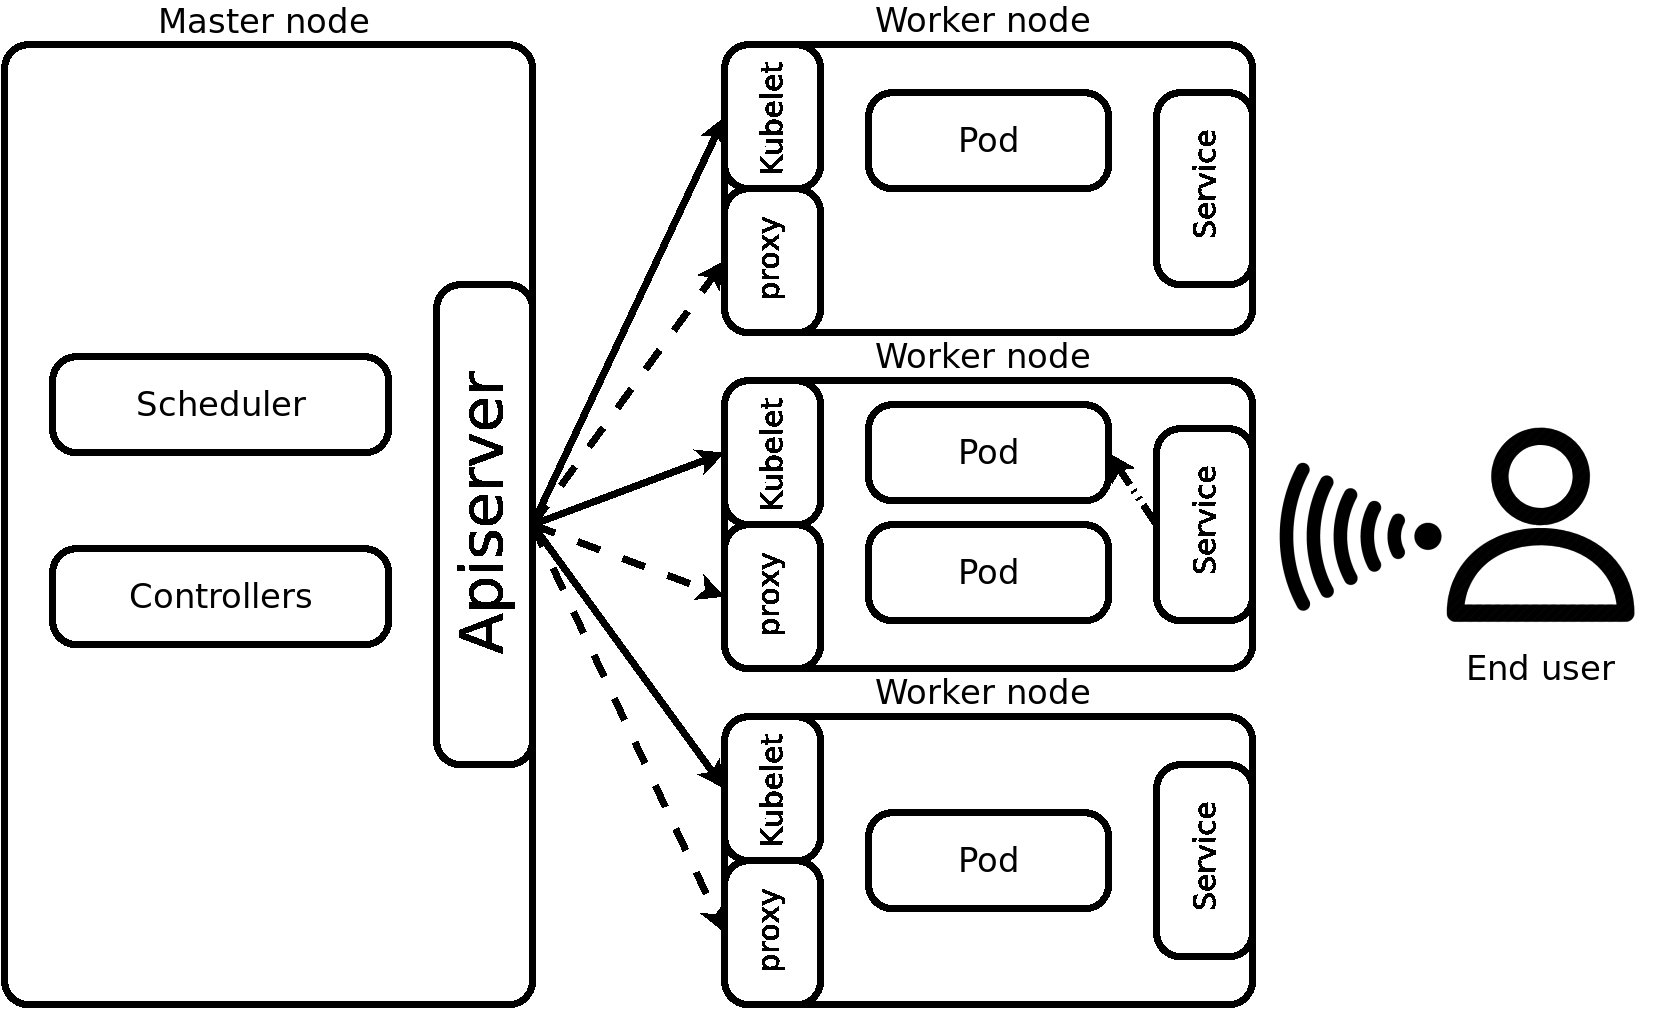
\includegraphics[width=\textwidth/2]{images/arch.png}
\begin{figure}[th]


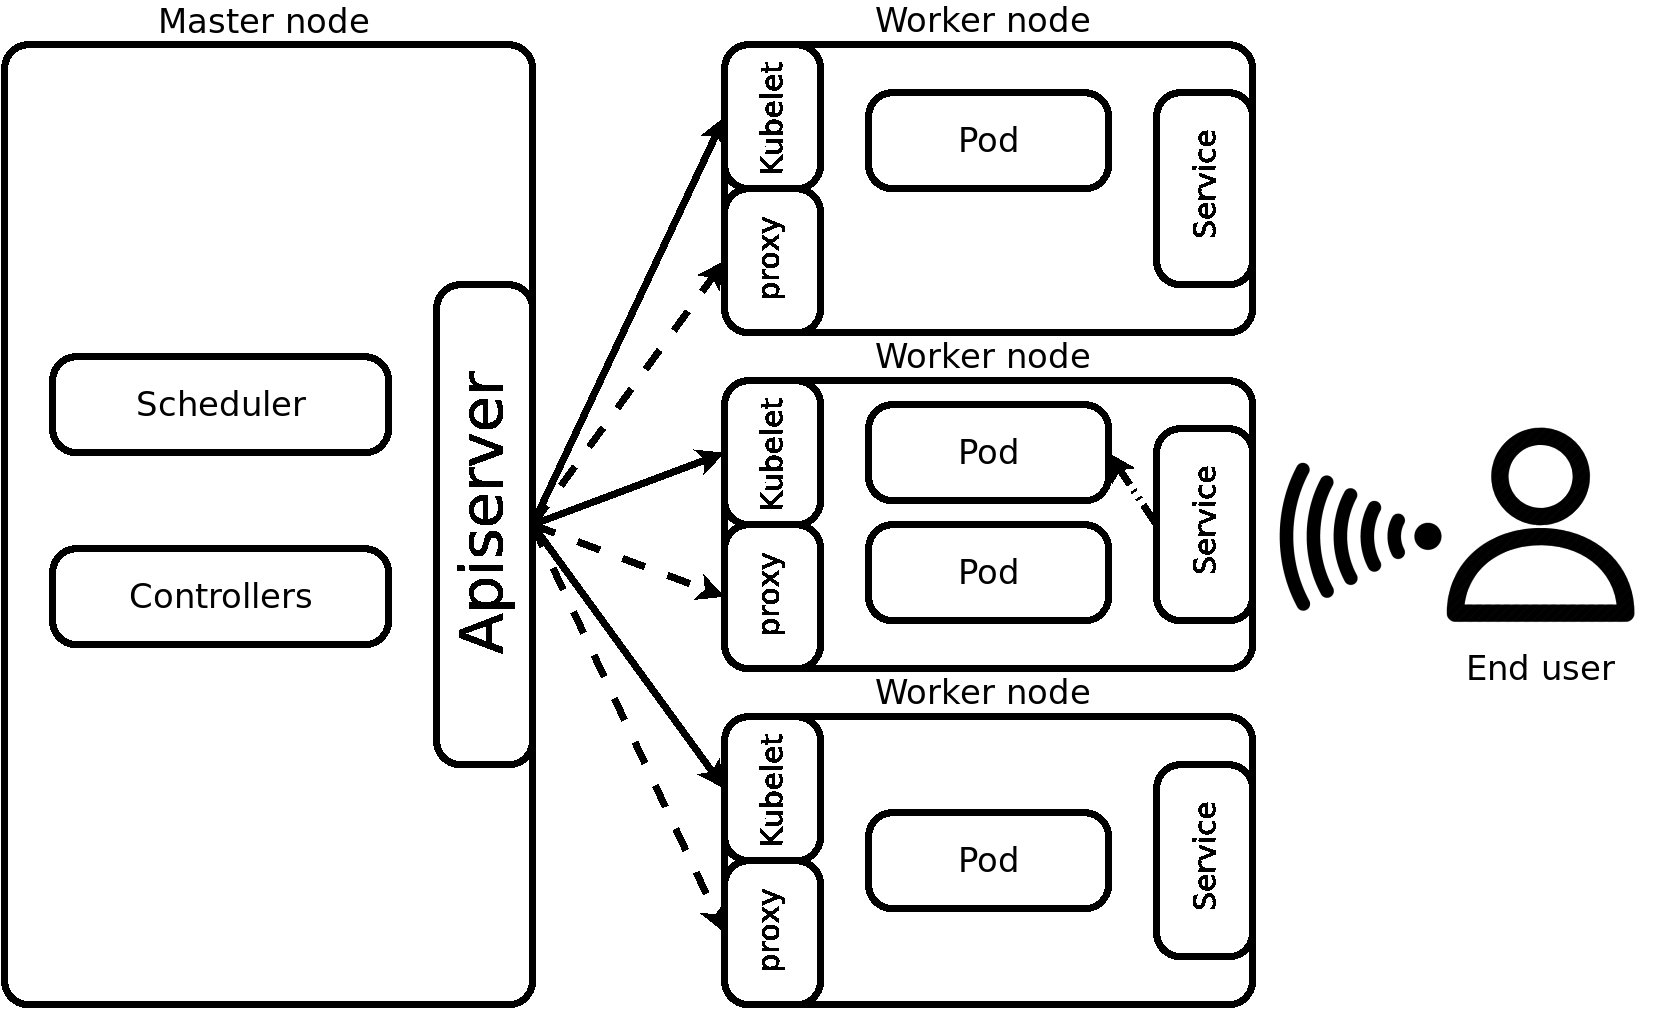
\includegraphics[width=0.51\textwidth]{images/arch.png}


\caption{Kubernetes architecture}
\end{figure}

%paragraph linking
\hskip .7em Kubernetes is an open-source container-based platform, this platform manages the orchestration of the service instances. A Kubernetes cluster consist of one master node and worker nodes, where a node does not necessarily refer to a physical machine, it can also be virtual. The master node is responsible for the management and monitoring of the cluster, the master node contains the deployment scheduler and controllers. \change{rephrase!} Meanwhile, the worker nodes are the actual resources of the platform, they run the user application inside containers created by the master node. 

In the following paragraphs we will refer to the master node as master and the worker node as node. 

%pods.
%deployment controllers.
Kubernetes runs containers in the form of pods, where a pod is a group of one or more containers. If a pod is consisting of more than one container, those containers can communicate internally using an isolated network\unsure{maybe it's over detailed}. The pods are created using a deployment controller located in the master node, and here we have to mention that the user is responsible of creating the deployment not the pods themselves. The automation of Kubernetes is responsible for the creation of the associated pods.

The master can schedule the pods in any of the available nodes. The pods have to communicate between each others and with users. Those communications are carried away using: 

\begin{itemize}
	\item Software Defined Networking(SDN) for pod-to-pod communication.
	\item Kube-proxy for the communication with the users, through K8's services.
\end{itemize}
%services
The main purpose of the service is connecting the users to exposed pods, by redirecting them to an available pod. The user will send the request to the service Ip address, then the service will choose one of the available pods in a resource pool \change{I will look for the correct name}\change{rephrase!} and looks for the Ip address of the pods in the Iptables. This selection is done in a random way or by using a load-balancer that will select the least used pod.
\begin{figure}[th]
\centering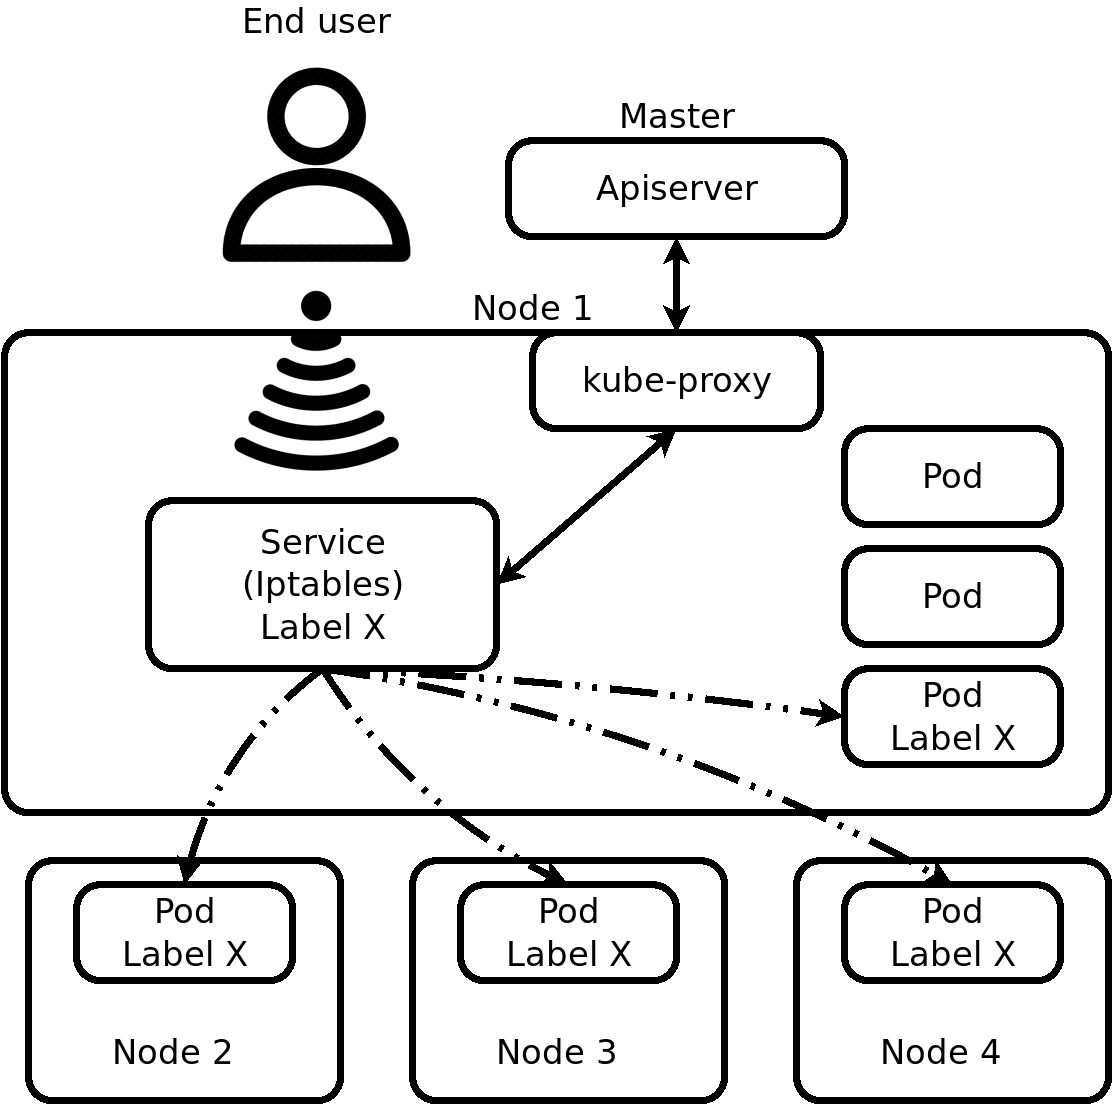
\includegraphics[width=0.33\textwidth]{images/svc.png}
\caption{Kubernetes service}
\end{figure}


\subsection{Kubernetes Advantages}
\begin{itemize}
\itemsep0em

\item{\bf Community} 
\hskip .7em Since Kubernetes is an open-source software, it's surrounded by a large-scale community consists of thousands of contributors from the industrial and research field, meeting and events, and forms to file issues and ask questions.

The support provided by this community ease the development of the software for everyone, where a number of features Kubernetes have today were developed through this community.  
\item {\bf Distribution} 
The fog architecture is based in wide distribution of plenty points of presence, spread over a geographical location. Kubernetes support building large clusters up to 5000 nodes and 150,000 pods, such support is ideal for fog distribution. 
\item {\bf Scalability} as a result of supporting large clusters, Kubernetes had to simplify the procedure of scaling the cluster. Adding new nodes to the cluster is as simple as running a join command, and the master node will take care of everything, without the need of the maintainer interference. 


\item {\bf Containerization} running applications inside containers is the new trend over Virtualization. Containerization outperform virtualization in lightweight \unsure{it can function as an noun checked}and in the facilitation of  the application's packaging, shipping, and deployment. That's why cloud platforms like K8's are built around this emerging concept, where the benefits of containers also applies in fog computing architecture.  

\item {\bf Deployment} Kuberentes deployment is done using deployment controllers located in the master node, these controllers receives user's request for new deployments and interpret them in terms of pods. The user will monitor the pods as a deployment, and any failure of a pod or a node would be automatically resolved without a manual intervention. 
\end{itemize}


\subsection{Kubernetes Disadvantages}

\hskip .7em While building our own test-bed cluster and running K8's on top of it, and by looking deeper in the code, we have spoted some of the drawbacks for running K8's for fog computing, the draw-backs can be summarized in the following: 

\begin{itemize}
\itemsep0em


\item {\bf Centralization}
K8's cluster is composed of master node and worker nodes, all the decision of the cluster are made by the master, and all the cluster controllers are located there. This imposes higher latencies when executing jobs like deploying a container, also heavy computations are done in the master node to take all the decision of the cluster.\change{rephrase!}  

\item{\bf Location awareness}
The fact that K8's does not support location awareness is not shocking, since K8's is a cloud platform. Yet the location awareness is the number one characteristic of fog computing \cite{Bonomi:2012:FCR:2342509.2342513}. 
The characteristic of location awareness is mainly required to allow the fog to trace the closest available resource, which will improve the latency.

\item {\bf Load balancing}
Load balancing in kubernetes is limited to external load balancers used in the cloud providers, since the fog is definitely not built in the cloud provider hardware then now load balancing options are not available for the fog.\unsure{need to check more}

\item {\bf Scheduling regardless the location}
neither the deployment of the containers, nor the scheduling of the incoming requests from the application users  is related to the location of the node. As a result we will end up by the jobs traversing more hops in the network before reaching the targeted nodes, which implies higher end-to-end latencies.\change{rephrase!}


\end{itemize}

%%%%%%%%%%%%%%%%%%%%%%%%%%%%%%%%%%%%%%%%%%%%%%%%%%%%%%%%%%% Roadmap %%%%%%%%%%%%%%%%%%%%%%%%%%%%%%%%%%%%%%%%%%%%%%%%%%%
\section{A Roadmap Towards Fog-aware Kubernetes}\label{road}

\subsection{The Decentralization}
\subsection{Location Awareness}
\subsection{Scheduling Schemes}

%%%%%%%%%%%%%%%%%%%%%%%%%%%%%%%%%%%%%%%%%%%%%%%%%%%%%%%%%%% Conclusion %%%%%%%%%%%%%%%%%%%%%%%%%%%%%%%%%%%%%%%%%%%%%%%%%%%
\section{Conclusion}

%%%%%%%%%%%%%%%%%%%%%%%%%%%%%%%%%%%%%%%%%%%%%%%%%%%%%%%%%%% Acknowledgments %%%%%%%%%%%%%%%%%%%%%%%%%%%%%%%%%%%%%%%%%%%%%%%%%%%
\section{Acknowledgments}

A polite author always includes acknowledgments.  Thank everyone,
especially those who funded the work. 

\section{Availability}


%\theendnotes


{\footnotesize \bibliographystyle{acm}
\bibliography{bibtex}
\newpage
\listoftodos[Notes]




\end{document}







